%! Suppress = MightBreakTexify
\documentclass{article}

\usepackage[utf8]{inputenc}
\usepackage[pagebackref,citecolor=blue,linkcolor=OliveGreen,urlcolor=Mahogany,colorlinks]{hyperref}
\usepackage[usenames,dvipsnames]{xcolor}
\usepackage{url}
\usepackage{amsmath}
\usepackage{amsfonts}
\usepackage{lmodern}
\usepackage{etoolbox}
\usepackage{amsthm}
\usepackage{color}
\usepackage{cleveref}
\usepackage{tikz}
\usepackage{csquotes}
\usetikzlibrary{positioning}

% coq
\usepackage{minted}
\usemintedstyle{emacs}

\crefformat{section}{\S#2#1#3} % see manual of cleveref, section 8.2.1
\crefformat{subsection}{\S#2#1#3}
\crefformat{subsubsection}{\S#2#1#3}

\newcommand{\TODO}[0]{{\color{red} TODO}}
\newcommand{\lrangle}[1]{\langle #1\rangle}
\newcommand{\RedPRL}{{\color{red} Red}PRL}

\usepackage[links]{agda}
\usepackage{newunicodechar}
\newunicodechar{λ}{\ensuremath{\mathnormal\lambda}}
\newunicodechar{←}{\ensuremath{\mathnormal\from}}
\newunicodechar{→}{\ensuremath{\mathnormal\to}}
\newunicodechar{∀}{\ensuremath{\mathnormal\forall}}
\newunicodechar{≡}{\ensuremath{\mathrel{=}}}



\title{Constructive Interpretations of HoTT (Draft)}
\author{Tesla Ice Zhang}

% allow multiple labels in displaymath
%! Suppress = Makeatletter
\makeatletter
\patchcmd{\mathdisplay}
{\let\label\label@in@display}{}
{}{\fail}
%! Suppress = Makeatletter
\makeatother

% new cmd
\newcommand\xtag{
\refstepcounter{equation}%
\;\;\text{(\theequation)}}
\newcommand{\refl}{\textsf{refl}}

\begin{document}
\maketitle

\tableofcontents

\section{Motivation}
\label{sec:motivation}

In the HoTT Book~\cite{hottbook},
the identity type is defined the same way as the one
in Martin-L\"{o}f Type Theory (hereafter as ``MLTT'')~\cite{MLTT},
but used differently (stated in Chapter 1 notes).
The elimination rule of the identity type is called \textbf{path induction},
but according to its definition we can tell
it's just another name of the MLTT \textbf J rule.

We distinguish them by calling the HoTT identity type the \textit{path type},
while the MLTT one as the \textit{identity type}.
The most notable difference is that the path type is
\textit{proof relevant} (implies the absence of
\textit{Axiom K}~\cite{AxiomK}).

By not providing a better definition of the path type,
we have to assume function extensionality as an axiom,
and we cannot compute transport on nontrivial paths.

To safely assume the univalence axiom, we need to avoid having Axiom K
in our type system.
Agda~\cite{Agda} implements~\cite{WithoutK} this via a flag \texttt{--without-K},
while in Coq~\cite{Coq}, Axiom K is not assumed.
Agda have further developed to have a without-K-compatible \textsf{Prop}
universe~\cite{PropWithoutK}, a without-K-compatible definitional equality
customization strategy~\cite{RewriteWithoutK}, and many other stuffs.
Another dependently-typed programming language similar to Agda,
Idris~\cite{Idris}, sticks to Axiom K and is
inconsistent~\cite{IdrisHoTT} with the univalence axiom.

Even we have ways to avoid Axiom K,
we are still missing a constructive version of function extensionality,
and we also cannot compute the univalence axiom.

\subsection{Introduction}
\label{subsec:introduction}

This note is about giving HoTT a completely constructive interpretation,
from an implementation and user-experience perspective.
The categorical models behind are discussed only when necessary.

By giving a constructive interpretation of HoTT,
these issues are addressed:

\begin{itemize}
\item The path type should be constructive --
  there need to be formation, introduction and
  elimination rules (\cref{sec:path}).
\item Transport should compute (\cref{subsec:coe}).
\item The univalence axiom (\cref{sec:ua}) and function extensionality
  (\cref{subsec:path-prop}) should compute.
\item Inductive types~\cite{Inductive} should allow \textbf{path constructors}
  to form \textit{higher inductive types} (\cref{sec:hit}).
\end{itemize}

This note assumes the reader to:

\begin{itemize}
\item Have brief understanding of HoTT.
\item Have basic understanding of dependent type programming and MLTT.
\end{itemize}
\section{Path types}
\label{sec:path}

To define Path constructively,
we may get some inspiration from its topological definition.
Open-up the \href{https://ncatlab.org/nlab/show/path}{``path'' segment in nLab},
there is a mathematical definition of a path, written as:

\[
  \mathbb I \rightarrow X
  \xtag
\]

Topologically, a path in a space $X$ is a continuous map
from an interval (denoted $\mathbb I$) to $X$.
Type theoretically, $\mathbb I$ and $X$ are types,
and $\mathbb I \rightarrow X$ is a function type from $\mathbb I$ to $X$.
As paths represent a relation \textit{between} two terms
(endpoints, but type theoretically),
these two terms should show up in the path type as well
(similar to MLTT identity type).
Therefore the formation rule for path types is naturally:

\[
  \cfrac{
    \Gamma \vdash X \ \textbf{type}
    \quad
    \Gamma \vdash a : X
    \quad
    \Gamma \vdash b : X
  }{\Gamma \vdash a =_X b \ \textbf{type}}
  \xtag
\]

Up to the time where this note is written,
everyone tries to define constructive HoTT defines path types this way.
They have different introduction and elimination rules,
but all of their introduction rules are
based on the interval type $\mathbb I$
and the elimination rules are slimiar to function application.

We can also define heterogeneous path types
(path between two terms of different types)
by changing the type $X$ into a type family $f$,
indexed by the interval type $\mathbb I$,
to allow paths between terms of different types:

\[
  \cfrac{
    \Gamma \vdash X \ \textbf{type}
    \quad
    \Gamma \vdash a : X
    \quad
    \Gamma \vdash b : X
    \quad
    \Gamma \vdash f : \mathbb I \rightarrow X
  }{\Gamma \vdash a =_f b \ \textbf{type}}
  \xtag \label{eqn:hetero-path}
\]

Heterogeneous paths are used in~\cref{subsec:path-hit}.

\subsection{Interval types}
\label{subsec:interval}

The interval type has very simple formation rule
and introduction rule:

\[
  \vdash \mathbb I\ \textbf{type}
  \xtag \quad
  \vdash \textsf 0 : \mathbb I
  \xtag \quad
  \vdash \textsf 1 : \mathbb I
  \xtag
\]

The programming language Arend~\cite{Arend} uses a different notation
(\textsf{left} instead of \textsf 0, \textsf{right} instead of \textsf 1)
for interval endpoints.
We will still use \textsf 0 and \textsf 1 when talking
about Arend for consistency.

The interval type do not yet have an elimination rule,
so we cannot have a predicate on an interval.

By this definition of interval, the path type can
have the following introduction rule
(definitional equality between term $a$ and $b$
is denoted as $a \equiv b$,
usually implemented via conversion checking or normalization):

\[
  \cfrac{
    \Gamma \vdash a =_X b \ \textbf{type}
    \quad
    \Gamma, i : \mathbb I \vdash t : X
    \quad
    (\lambda i. t) \ \textsf 0 \equiv a
    \quad
    (\lambda i. t) \ \textsf 1 \equiv b
  }{
    \Gamma \vdash \lrangle i t : a =_X b
  }
  \xtag
\]

Heterogeneously:

\[
  \cfrac{
    \Gamma \vdash a =_F b \ \textbf{type}
    \quad
    \Gamma, i : \mathbb I \vdash t : F \ i
    \quad
    (\lambda i. t) \ \textsf 0 \equiv a
    \quad
    (\lambda i. t) \ \textsf 1 \equiv b
  }{
    \Gamma \vdash \lrangle i t : a =_F b
  }
  \xtag
\]

The above definition is used in Cubical Type Theory~\cite{CCHM,CHM}
(hereafter as CTT), Cartesian Cubical Type
Theory~\cite{CCTT,CCTT2,CHTT} (hereafter as CCTT).
There are three usable implementations of CTT described in~\cite{CHM},
including cubicaltt~\cite{CubicalTT},
mlang~\cite{Mlang} and Cubical Agda~\cite{CubicalAgda}.
For CCTT, there are two, including
redtt~\cite{RedTT} (somehow supersedes and deprecates
\RedPRL~\cite{RedPRL}) and yacctt~\cite{YaccTT},
which implement different variations of CCTT.

The syntax is intentionally made similar to a lambda abstraction,
as the introduction rule is the same as lambda abstraction with
additional two definitional equalities required.
The elimination rule for a path is therefore similar to an application,
with two additional reduction rules -- applying an interval $i$ to
an arbitrary term whose type is known to be a path type $a =_X b$
will reduce to $a$ if $i \equiv \textsf 0$ or $b$ if $i \equiv \textsf 1$:

\[
  \cfrac{
    \Gamma \vdash p : a =_X b
  }{
    \Gamma \vdash p\ \textsf 0 \equiv a
    \quad
    \Gamma \vdash p\ \textsf 1 \equiv b
  }
  \xtag \label{eqn:path-app}
\]

Rule~\ref{eqn:path-app} holds even if $p$ is a neutral term,
or a contructor (in case there's path constructors,
introduced in~\cref{subsec:path-hit}).
Therefore constructor application can be redex as well.

CTT and CCTT (and many other variations) have different primitive
operations defined for the interval type,
we discuss this later in~\cref{sec:kan}.

Arend on the other hand defines a primitive operator \textsf{path}
as the introduction rule for path:

\[
  \cfrac{
    \Gamma \vdash X \ \textbf{type}
    \quad
    \Gamma \vdash t : \mathbb I \rightarrow X
  }{
    \Gamma \vdash \textsf{path} \ t : (t \ \textsf 0) =_X (t \ \textsf 1)
  }
  \xtag
\]

The elimination of paths is still similar to CTT or CCTT.

CTT and CCTT do not support creating paths between intervals,
while Arend do.
Thus the following judgement holds in Arend, say,
that there exists a path between \textsf 0 and \textsf 1:

\[
  \vdash \textsf{path}\ (\lrangle i i) : \textsf 0 =_{\mathbb I} \textsf 1
  \xtag \label{eqn:0-1-arend}
\]

This does not mean that \textsf 0 is identical to \textsf 1.
They are not equivalent definitionally, but propositionally.
Here's the concrete syntax of~\ref{eqn:0-1-arend} in Arend:

\begin{minted}{arend-lexer.py:ArendLexer -x}
  \func interval-path : left = right => path (\lam i => i)
\end{minted}

\subsubsection{Interval operations}

Different model defines different operations on the $\mathbb I$ type.

\TODO

\subsection{Path properties}
\label{subsec:path-prop}
\input{latex/path-properties}

\subsection{Transport}
\label{subsec:coe}

The idea of \textit{type-safe coercion} is like
casting a variable of type $A$ to type $B$ by providing a proof
of $A =_{\mathcal U} B$:

\[
  \textsf{coe} : A =_{\mathcal U} B \rightarrow A \rightarrow B
  \xtag \label{eqn:coe-a-b-id}
\]

Bringing in the idea of path types,
assuming $p : A =_{\mathcal U} B$, by~\ref{eqn:path-app}
we know that $p~\textsf 0 \equiv A$ and
$p~\textsf 1 \equiv B$,
so~\ref{eqn:coe-a-b-path} is effectively the same
as~\ref{eqn:coe-a-b-id}:

\[
  \textsf{coe} : (p : A =_{\mathcal U} B) \rightarrow p~\textsf 0
  \rightarrow p~\textsf 1
  \xtag \label{eqn:coe-a-b-path}
\]

The return type of \textsf{coe} can be generalized over
the interval on the input path:

\[
  \textsf{coe} : (p : A =_{\mathcal U} B) \rightarrow p~\textsf 0
  \rightarrow (i : \mathbb I) \rightarrow p~i
  \xtag \label{eqn:coe-a-b-path-gen}
\]

\ref{eqn:coe-a-b-path-gen} is known as the ``generalized transport''
operation, denoted as \textsf{coe} in Arend and CCTT,
and \AgdaFunction{transp} in CTT.
We use \textsf{coe} to refer to this general concept for consistency.
And by the way,
Arend's \textsf{coe} takes function over interval instead
of a path as its first argument:

\[
  \textsf{coe} : (p : I \rightarrow \mathcal U)
  \rightarrow p~\textsf 0
  \rightarrow (i : \mathbb I) \rightarrow p~i
  \xtag
\]

We can state that $\textsf{coe}~p~a~\textsf 0$ will give $a$ back
(i.e. reduce to $a$).

Right now there is neither nontrivial path nor path on types,
while transport along identity paths is just a fancy version
of the identity function, thus we do not need to worry about the
computation of \textsf{coe} yet.
We further discuss \textsf{coe} in~\cref{sec:ua}.

In CTT and CCTT, we cannot transport along paths between paths,
but it's not the case in Arend.
Arend uses \textsf{coe} to prove path symmetry and transitivity.
Here's a proof, assuming three inhabitants $a, b, c$ of type $A$
and the trivial path $\refl_a : a =_A a$:

\[
  \cfrac{
    \Gamma \vdash p : a =_A b
  }{
    \Gamma \vdash (\textsf{coe}
    (\lambda i. (p~i =_A a))~\refl_a~\textsf 1)
    : b =_A a
  }
  \xtag \label{eqn:arend-proof-sym}
\]

In Arend's concrete syntax, path application is not
$p~i$ but $p~@~i$ and lambda abstraction is not $\lambda x.y$ but
$\backslash{}\textsf{lam}~x \Rightarrow y$.
Therefore the concrete syntax of~\ref{eqn:arend-proof-sym} in Arend is:

\begin{minted}{arend-lexer.py:ArendLexer -x}
  \func sym {A : \Type} {a b : A} (p : a = b) : b = a =>
    coe (\lam i => p @ i = a) idp right
\end{minted}

What happened in~\ref{eqn:arend-proof-sym} is that we transported
along the following interval lambda:

\[
  f = \lambda i. (p~i =_A a)
  \xtag
\]

As $p : a =_A b$, we have
$(f~\textsf 0) \equiv (p~\textsf 0 =_A a) \equiv (a =_A a)$ and
$(f~\textsf 1) \equiv (p~\textsf 1 =_A a) \equiv (b =_A a)$,
so $f$ is similar to a path $(a =_A a) =_{\mathcal U} (b =_A a)$.
By providing a proof $\refl_a$ of $a =_A a$,
we obtain the proof of the right hand side of $f$, which is $b =_A a$.
The proof of transitivity is similar, as in~\ref{eqn:arend-proof-trans}.
Analyzing how it works is left as an exercise.

\[
  \cfrac{
    \Gamma \vdash p : a =_A b
    \quad
    \Gamma \vdash q : b =_A c
  }{
    \Gamma \vdash (\textsf{coe}
    (\lambda i. (a =_A q~i))~p~\textsf 1)
    : a =_A c
  }
  \xtag \label{eqn:arend-proof-trans}
\]

It looks like the following in Arend:

\begin{minted}{arend-lexer.py:ArendLexer -x}
  \func trans {A : \Type} {a b c : A}
              (p : a = b) (q : b = c) : a = c =>
    coe (\lam i => a = q @ i) p right
\end{minted}

\subsection{Fillers}
\label{subsec:fill}

Recall~\ref{eqn:arend-proof-sym}, we can take the \textsf 1 argument away from
the applicaiton to \textsf{coe}:

\[
  \cfrac{
    \Gamma \vdash p : a =_A b
  }{
    \Gamma \vdash (\textsf{coe}
    (\lambda i. (p\ i =_A a)) \ \refl_a)
    : \mathbb I \rightarrow b =_A a
  }
  \xtag \label{eqn:coe-a-b-path-gen-eta}
\]

Also, we know that the term $t = \textsf{coe} (\lambda i. (p\ i =_A a)) \ \refl_a$
satisfies $t\ \textsf 0 \equiv \refl_a$.
Recall $t\ \textsf 1 : b =_A a$,
we have the following definitional equalities:

\[
  t\ \textsf 0\ \textsf 0 \equiv a \xtag \quad
  t\ \textsf 0\ \textsf 1 \equiv a \xtag
\]
\[
  t\ \textsf 1\ \textsf 0 \equiv b \xtag \quad
  t\ \textsf 1\ \textsf 1 \equiv a \xtag
\]

Here we can see $t$ as a higher-dimensional path,
as it's like a function taking more than one intervals,
while satisfying definitional equalities for all permutations of the endpoints.
Since it's two-dimensional, we call $t$ a \textit{square},
of the shape in~\cref{fig:filler}.

\begin{figure}
\begin{center}
  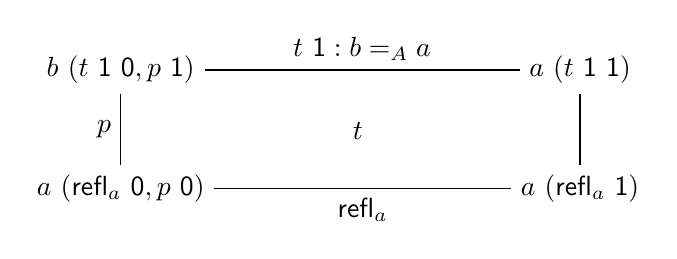
\begin{tikzpicture}[node distance=1.5cm]
    \node(1) {$b$ ($t\ \textsf 1\ \textsf 0, p\ \textsf 1$)};
    \node(2) [right=4cm of 1] {$a$ ($t\ \textsf 1\ \textsf 1$)};
    \node(4) [below of=1] {$a$ ($\refl_a\ \textsf 0, p\ \textsf 0$)};
    \node(3) [below of=2] {$a$ ($\refl_a\ \textsf 1$)};
    \draw (1) -- (2) node[midway,above] {$t\ \textsf 1 : b =_A a$};
    \draw (1) -- (4) node[midway,left ] {$p$};
    \draw (3) -- (2);
    \draw (3) -- (4) node[midway,below] {$\refl_a$};
    \path (1) -- (3) node[midway] {$t$};
  \end{tikzpicture}
\end{center}
\caption{Filler for symmetry}
\label{fig:filler}
\end{figure}

Squares can be seen as paths between paths.
We can generalized this terminology to form topological shapes in any dimensions.
Paths between paths are \textit{homotopies} in HoTT,
while we informally call $t$ a \textit{filler} of the above square
when talking about constructive interpretations.

Note: fillers might be either paths or functions over intervals,
so we can also say $\textsf{path} \ t$ is a filler of the same square.
We use the term just to follow the convention.


By the above constructive path type,
we can extend inductive types with path constructors.
Recall that a constructor of an inductive type $T$ is
similar to a function whose return type is $T$,
but does not reduce.

\TODO
\section{Kan operations}
\label{sec:kan}

In~\cref{subsec:coe}, we have seen an operation on paths,
that is \textsf{coe}, which returns a path~\footnote
{It's not actually a path in Arend, but a function over intervals.
  We can say it's \textit{almost} a path.}.
Since it returns a path, we may wonder how is the returned path
represented internally.
Ideally, we want \textsf{coe} to be a built-in but reducible function,
which means that it \textbf{computes} when fully applied.
Unfortunately, \textsf{coe} in Arend only computes in certain hard-coded cases,
which is not ideal.
There is a more general operation in CTT and CCTT which allows computation
on path operations, namely \textit{Homogenous composition}.

The idea is in one sentence:

\begin{displayquote}
  For any n-dimensional cube, it has $2 \times n$ faces.
  If we can construct $2 \times n - 1$ of them,
  the last one face can be obtained by doing a homogenous composition.
\end{displayquote}

In case it's two-dimensional, the cube becomes a square,
and it has four faces, which are all one-dimensional paths.
If we can have three of these paths,
we can obtain the last path via homogenous composition.
We can graph this process, as in~\cref{fig:simple-comp}
(assuming $\vdash a, b, c, d : A$).

\begin{figure}
\begin{center}
  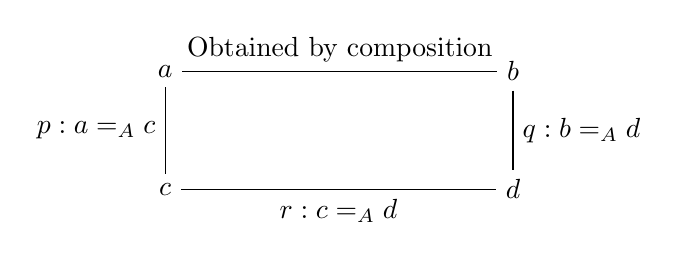
\begin{tikzpicture}[node distance=1.5cm]
    \node(1) {$a$};
    \node(2) [right=4cm of 1] {$b$};
    \node(4) [below of=1] {$c$};
    \node(3) [below of=2] {$d$};
    \draw (1) -- (2) node[midway,above] {Obtained by composition};
    \draw (1) -- (4) node[midway,left ] {$p : a =_A c$};
    \draw (3) -- (4) node[midway,below] {$r : c =_A d$};
    \draw (2) -- (3) node[midway,right] {$q : b =_A d$};
  \end{tikzpicture}
\end{center}
\caption{Simple composition}
\label{fig:simple-comp}
\end{figure}

This looks very similar to~\cref{fig:filler}
if we substitute $a$ with $b$ and $b, c, d$ with $a$.
We can also prove path composition by substituting $a$ with $c$.

Here's the surface syntax of homogenous composition.
In~\cite{CCHM}, there are two basic structures that the composition operation
is based on:

\begin{align*}
  \varphi &= (i=\textsf 0) \mid (i=\textsf 1)
  & \xtag \\
  u &= [ \; \varphi_1 \mapsto t_1,
      \dots, \varphi_n \mapsto t_n \; ]
  & \xtag
\end{align*}

$\varphi$ is called the \textit{Face lattice},
which stands for a constraint that specifies a face.
$u$ is a list of face-term pair $\varphi \mapsto t$,
where each pair specifies a term $t$ for a face $\varphi$.
Thus we can describe an open shape via $u$.

The composition operation is defined as following:

\newcommand{\comp}{\textsf{comp}}

\[
  \cfrac
  {\Gamma, i : \mathbb I \vdash A \quad
    \Gamma, \varphi, i : \mathbb I \vdash u : A \quad
    \Gamma \vdash a_0 : A(\textsf 0)[ \varphi \mapsto u(\textsf 0) ]}
  {\Gamma \vdash \comp^i~A~[ \varphi \mapsto u ]~a_0 :
    A(\textsf 1)[ \varphi \mapsto u(\textsf 1) ]}
\]

In naturally language, given
$A$ -- a type indexed by $\mathbb I$,
$a_0$ -- a term for the bottom face of the cube,
$u$ -- a list of face-term pairs representing all the faces except
$a_0$ and the top-missing face.
Then, $\comp^i~A~[ \varphi \mapsto u ]~a_0$ produces the top face.

In CCTT, there is another variation of $\varphi$:

\[
  \varphi = \dots \mid (i = j)
  \xtag
\]

This face specifies a diagonal,
giving us more computation rules.

\section{Univalence}
\label{sec:ua}

\TODO


\bibliography{ref}
\bibliographystyle{alpha}

\end{document}
